\documentclass{article}
\usepackage{luatextra}
\usepackage{polyglossia}
\usepackage{ulem}
\usepackage{framed}
\usepackage{color}
\usepackage{geometry}
\usepackage{amsmath}
\usepackage{unicode-math}
\usepackage{hyperref}
\usepackage{latexsym}
\usepackage{graphicx}

\usepackage{ifluatex}
\ifluatex
  \usepackage{pdftexcmds}
  \makeatletter

  \let\pdfstrcmp\pdf@strcmp
  \let\pdffilemoddate\pdf@filemoddate
  \makeatother
\fi
\usepackage{svg}

\setmathfont{xits-math.otf}

\setmainlanguage{french}
\setmainfont{Latin Modern Roman}

\geometry{margin={1in,1in}}

\setlength{\parskip}{1em}

\newcommand\image[2]{
\directlua{
local image = img.scan({filename = "#1"})

image.height = image.height * #2
image.width  = image.width  * #2

node.write(img.node(image))
}
}

\author{MIAOU Is An Open Umbrella\\Nassim Bounouas\\Guillaume Casagrande\\Julien Lemaire\\Pierre-Emmanuel Novac}
\title{\vspace{-1cm}Rapport Niveau 3 --- Projet BRAINF-CK}

\begin{document}

\maketitle

\section{Introduction}

    Ce rapport présente la troisième version de notre interpréteur Brainfuck. Elle regroupe les fonctionnalités des niveaux 1, 2 et 3 (les modifications sont visibles dans la Fig.1).
    Le niveau 3 apporte des fonctionnalités et des améliorations qui facilitent le travail des développeurs. Nous leur offrons la possibilité de suivre les performances de leur programme à l’aide de métriques portant par exemple sur le nombre d'instructions exécutées ou le temps d'exécution. Nous proposons aussi un moyen efficace de suivre l’exécution du programme à l'aide d'un fichier de journalisation. Il permet d’identifier les éventuelles erreurs plus rapidement. Ensuite, deux nouvelles fonctionnalités améliorent la clarté d'un programme Brainfuck. Il est dorénavant possible d’ajouter des commentaires et des espaces à l’intérieur du programme écrit en Brainfuck. Cela facilite la lisibilité et la compréhension du code. Notre interpréteur est aussi capable de prendre en compte des macros. Celles-ci permettent d’écrire un code plus compact. Enfin, l'implémentation des sauts reposent désormais sur une table de saut plutôt qu'un parcours linéaire des instructions.

    Avant le niveau 3, nous avons mis en place une machine virtuelle possédant une mémoire pour stocker les données du programme. Notre machine permet l'exécution des instructions d'incrémentation, de décrémentation,de déplacement à gauche et à droite dans la mémoire, d'entrée et de sortie, le saut conditionnel en avant et le retour en arrière conditionnel telles que définies dans le langage Brainfuck. Il prend également en charge différents types de syntaxe : les syntaxes courte, longue et sous forme d’image. Pour passer de l’une à l’autre, un traducteur est mis à disposition. Il est aussi possible de vérifier la cohérence des sauts d’un programme Brainfuck. Ces deux dernières fonctionnalités sont activables par le biais d'options lors de l'appel de l'exécutable (\texttt{-{}-translate}, \texttt{-{}-rewrite}, \texttt{-{}-check} ...).

\begin{figure}[!ht]
	\centering
	\includegraphics[scale=0.6]{svgL3/diagClass}
	\caption{Diagramme de classes}
\end{figure}

\section{Commentaires et indentation}
    Le langage Brainfuck a été inventé pour devenir un véritable casse-tête pour les programmeurs. Avec ses 8 symboles disponibles, il n’est pas intuitif à utiliser et les programmes deviennent rapidement verbeux et peu lisibles. C’est pourquoi notre interpréteur est maintenant capable de prendre en compte l’indentation et les espaces. Il est donc possible de délimiter visuellement des blocs de code comme avec de nombreux autres langages et d’ajouter des espaces à l’intérieur d’une ligne écrite en syntaxe courte pour l’aérer. Le caractère croisillon permet l'insertion d'un commentaire en fin de ligne. La ligne sera lue comme si le commentaire n’existait pas. Le programmeur peut donc ajouter des annotations au programme pour expliquer son fonctionnement par exemple.

    Aucune classe n’a été ajoutée pour réaliser cette fonctionnalité. Nous avons directement modifié l'analyseur syntaxique : la classe \texttt{InstructionParser}. Pour rappel, cette classe analyse le contenu du fichier à interpréter afin d’obtenir une liste d’instructions. C’est donc dans cette classe que nous avons ajouté un filtre sur chaque ligne du programme lu. Lors de la lecture d’un croisillon, le contenu suivant celui-ci est ignoré par extraction de la sous-chaîne précédant le caractère. Pour supprimer les espaces et les tabulations, nous avons appliqué un \texttt{trim()} sur les chaînes de caractères. Cette méthode supprime les espaces situés en début et en fin de chaîne.

\section{Journalisation}
    Un programme Brainfuck est une suite d’instructions très simplistes. Ainsi les programmes deviennent rapidement verbeux . Pour éviter d’écrire des programmes trop long, il faut être minutieux et malin. Par exemple, pour écrire les lettres « x » et « y » avec du Brainfuck, il est ingénieux d’utiliser la même case mémoire pour afficher une lettre, puis l’autre. En effet, il manque qu’une seule incrémentation pour passer du « x » au « y ». Si un « a » doit être ajouté, il semble logique d’utiliser une nouvelle case en mémoire. Ce type de raisonnement devient rapidement compliqué lorsqu’il faut écrire de longs programmes. Si le résultat n’est pas celui attendu, il devient alors pratiquement impossible de déterminer la source de l’erreur. C’est pourquoi nous avons ajouté une nouvelle fonctionnalité à notre interpréteur Brainfuck : un journal. Celui-ci recense les étapes de l’exécution, facilitant le débogage d'un programme. Il suffit de vérifier dans le journal si chaque étape était bien celle attendue. Celles-ci sont numérotées : cette information est la première qui s’affiche dans le journal. Ensuite, un deuxième nombre est affiché : c’est la position du pointeur d’exécution. Il est utilisé dans notre programme pour parcourir la liste des instructions. Par la suite, le journal écrit le nom de l’instruction exécutée. Celle-ci est écrite en syntaxe longue pour plus de lisibilité. L’information inscrite juste après correspond à la position du pointeur de données. Il permet au développeur de savoir sur quelle case mémoire il est en train de travailler. Enfin, l’intérêt principal du journal réside dans la dernière donnée affichée : la mémoire. Une fois l’instruction exécutée, il devient facile de voir quelle case mémoire a été impactée grâce à la liste des états de chaque élément de la mémoire.

    Afin de créer ce journal, nous avons conçu une nouvelle classe : \texttt{Logger}. Un objet \texttt{Logger} est instancié dans la classe \texttt{Main} lorsque le paramètre \texttt{-{}-trace} est passé par l’utilisateur. La méthode principale de cette classe est \texttt{logStep}. C’est elle qui construit les lignes qui seront affichées dans le journal. Cette méthode prend en paramètre la position du pointeur d’exécution, la dernière instruction exécutée et la machine (afin de récupérer la position du pointeur de données et la mémoire). \texttt{logStep} est appelée dans l’interpréteur pour chaque instruction. Ainsi, lorsque l’interpréteur analyse une nouvelle instruction, le \texttt{Logger} est capable de stocker les données correspondant à la dernière action réalisée. Il est à noté que \texttt{Logger} utilise une classe déjà présente dans le projet : \texttt{WriteTextFile}. Sa méthode \texttt{write} écrit dans un fichier chaque entrée du journal. Ce fichier porte le nom du programme Brainfuck dont l'extension \texttt{.bf} a été remplacée par \texttt{.log}.

    Cette nouvelle classe a l'avantage d’être isolée du reste du programme. Nous l’appelons dans l'interpreteur sans qu’elle perturbe l’exécution du programme. Nous aurions pu directement ajouter les méthodes de la classe \texttt{Logger} dans la classe \texttt{Interpreter}. Or, nous avons trouvé ce choix peu orienté objet. Une classe a toujours un but. Celui de l’interpréteur est d’interpréter du Brainfuck, non pas de générer un journal. Il semblait donc judicieux d’ajouter une nouvelle classe qui aurait ce rôle.


\section{Table de sauts}

    En programmation, la possibilité de contrôler le flot d'exécution est primordial. Le langage Brainfuck comme la plupart des langages de programmation propose des structures de contrôle et plus exactement des instructions de saut conditionnel. Ces instructions ont la particularité d'influencer l'ordre de l'exécution en fonction de conditions pré-établies.


    Dans notre cas, les deux instructions en question sont \texttt{JUMP} et \texttt{BACK}. Le \texttt{JUMP} renvoyant le pointeur d'exécution à l'instruction \texttt{BACK} qui lui est associée si le contenu de la case mémoire actuelle est 0. Dans le cas contraire, le flot d'exécution n'est pas modifié. Le \texttt{BACK} adopte le même comportement de manière à obtenir un comportement de boucle tant que le contenu de la case mémoire pointée est différent de 0.


    La première version de notre interpréteur implémentait ce mécanisme de manière naïve en se contentant de déplacer le curseur instruction après instruction sans les exécuter lorsque nous étions dans le cas d'un saut conditionnel. Notre nouvelle version a la capacité de se rendre directement sur l'instruction de contrôle associée lors d'un saut. Cette amélioration repose sur l'ajout d'une table de sauts conditionnels, générée lors du chargement en mémoire de notre programme. Cette table de sauts enregistre la position de chaque instruction \texttt{JUMP}/\texttt{BACK} et l'associe à la position de l'instruction qui lui est liée.


    En d'autres termes, supposons le programme Brainfuck suivant :


 \begin{verbatim}
    ++[>+<-]
\end{verbatim}


    Ici, nous incrémentons la valeur de la première case mémoire jusqu'à ce qu'elle contienne 2, vérifions que le contenu de cette dernière est différent de 0, déplaçons le pointeur mémoire vers la droite, incrémentons la seconde case mémoire, revenons sur la première et la décrémentons.


    Ce programme est équivalent au pseudo-code suivant :

 \begin{verbatim}   

    x = 0

    Pour i allant de 2 jusqu'à 1 (inclus)

        x + 1

\end{verbatim}



    Dans notre version naïve des sauts conditionnels, nous exécutions une première fois la boucle \texttt{[>+<-]} puis parcourions cette même boucle en sens inverse sans en exécuter les instructions jusqu'à revenir à l'instruction de JUMP. Dans la version améliorée, une fois l'instruction \texttt{BACK} atteinte, nous revenons directement au \texttt{JUMP} si le contenu de la case pointée est différent de 0.


    Nous avons fait le choix de créer une nouvelle classe nommée \texttt{JumpTable} afin de générer cette table en même temps que la liste d'instructions dans la classe \texttt{InstructionParser}. De cette manière, lorsque nous communiquons à l'interpréteur la liste d'instructions à exécuter, nous lui communiquons indépendamment la table de saut et celle-ci permet un contrôle extérieur à liste.


    La table de saut est générée en même temps que la liste, lorsqu'une instruction \texttt{JUMP} est rencontrée sa position est déposée sur une pile de manière à récupérer la position du dernier \texttt{JUMP} lorsqu'un \texttt{BACK} est rencontré pour associer les deux positions dans une table de hachage.



    Notre choix technique a été guidé par la volonté d'avoir un unique objet gérant la table de saut conditionnel. Cette table ne contenant qu'un ensemble de type primitif, il nous a semblé judicieux de représenter la table de la manière la plus simple possible. Cette fonctionnalité est donc centralisée ce qui nous donne une unique référence pour tous nos sauts.


    Le choix de la pile pour la gestion des \texttt{JUMP} a été retenu car elle permet aussi de contrôler la cohérence du programme. Si nous arrivons à la fin des instructions et qu'elle n'est pas vide, alors au moins une instruction \texttt{JUMP} n'a pas d'instruction \texttt{BACK} correspondante. Dans le cas où nous rencontrons une instruction \texttt{BACK} et que la pile est vide, cela signifie qu'une boucle est fermée alors qu'elle n'a pas été ouverte.


    Ce comportement de vérification de la cohérence des sauts peut être considéré comme un avantage de notre implémentation. Cependant, notre modèle présente un inconvénient à savoir un fort couplage entre notre interpréteur et notre table de saut. Les valeurs utilisées dans la table de saut sont obtenues lors de l'analyse du programme et correspondent à l'indice des instructions. Elles sont par la suite utilisées par l'interpréteur pour le suivi de l’exécution du programme.

\section{Métriques}


    Depuis le début de notre projet, nous contrôlons la sortie d'un programme : le résultat obtenu est-il celui attendu ? Nous sommes capables de voir si l' implémentation d'un algorithme en Brainfuck est fonctionnelle mais nous ne pouvons pas juger de son efficacité. De ce fait, nous ne pouvions pas comparer deux programmes Brainfuck ayant la même finalité mais deux implémentations différentes. De plus, nous ne pouvions pas directement constater les améliorations apportées à notre système lors de son exécution.


    Afin de remédier à ces lacunes, un système de mesure a été intégré à notre application. Au total 6 points de mesure sont présents : 


\begin{itemize}
	\item \texttt{PROG\_SIZE} représente le nombre d'instructions dans le programme
	\item \texttt{EXEC\_TIME} correspond au temps d'exécution du programme en millisecondes
	\item \texttt{EXEC\_MOVE} correspond au nombre de déplacements du pointeur d'exécution
	\item \texttt{DATA\_MOVE} correspond au nombre de déplacements du pointeur sur la mémoire
	\item \texttt{DATA\_READ} correspond au nombre de lecture de la mémoire
	\item \texttt{DATA\_WRITE} correspond au nombre d'écriture en mémoire
\end{itemize}

    L'ensemble de ces valeurs est affiché à la fin de l'exécution du programme.



    Concernant l'aspect technique, nous avons fait le choix d'une énumération nommée \texttt{Metrics} contenant nos métriques. Tous les points de mesure ayant en commun de contenir une unique valeur numérique entière, nous avons placé un attribut de type \texttt{long} correspond à la valeur mesurée et ce sont les manières d'accéder à cette valeur qui diffèrent selon la métrique. 


    Lorsque nous calculons \texttt{PROG\_SIZE}, c'est l'interpréteur qui insère la taille de la liste d'instructions dans l'attribut.


    Dans le cas de la mesure \texttt{EXEC\_TIME}, au début de l'exécution l'attribut contient l'horodatage du début d'exécution et à la fin de l'exécution, sa valeur est remplacée par la différence entre le premier horodatage stocké et l'horodatage courant. Cette mesure justifie l'utilisation du type \texttt{long} puisqu'un temps en millisecondes pourrait dépasser la capacité de stockage du type \texttt{int}.


     L'interpréteur se charge d'incrémenter la valeur de la mesure  \texttt{EXEC\_MOVE} à chaque exécution d'instructions.


    En ce qui concerne les mesures \texttt{DATA\_MOVE}, \texttt{DATA\_WRITE} et \texttt{DATA\_READ}, elles sont contrôlées directement depuis les instructions agissant sur l'action mesurée.


    Etant donné que le comportement ajouté aux instructions se trouve être redondant pour certaines d'entres elles, l'arborescence des instructions a été étendue. Les classes d'instruction \texttt{Left} et \texttt{Right} dérivent de \texttt{MoveCursor}, qui incrémente \texttt{DATA\_MOVE}. Les classes d'instruction \texttt{In}, \texttt{Incr} et \texttt{Decr} dérivent de \texttt{WriteMemory} qui incrémente \texttt{DATA\_WRITE} et les classes d'instruction \texttt{Out}, \texttt{Jump} et \texttt{Back} dérivent de \texttt{ReadMemory} qui incrémente \texttt{DATA\_READ}.

\begin{figure}[!hb]
        \centering
        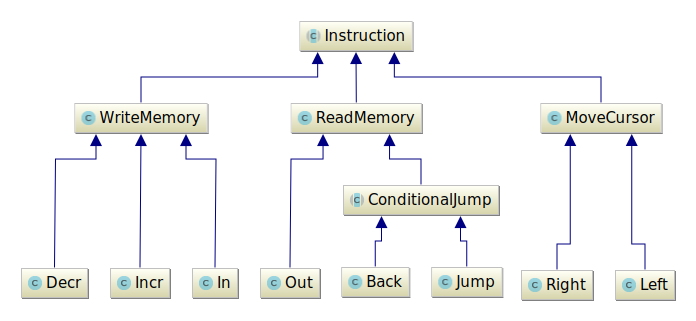
\includegraphics[scale=0.6]{svgL3/instructions}
        \caption{Hiérarchie des classes d'instruction}
\end{figure}


    Dans ce cas, étant donné que le nombre d'instruction est limité et que la liaison avec les métriques repose sur une ligne de code, nous aurions pu nous passer de ces ajouts qui peuvent paraître lourd.

    Ils ont tout de même l'avantage de clarifier le type d'instruction et permet d'éviter de se soucier de la gestion des métriques dans chacune des instructions implémentées.

    A l'appel de chacune de ces instructions, la valeur correspondant à la mesure est incrémentée par le biais d'un appel à la méthode de leur classe mère.


    L'implémentation par le biais d'une énumération permet de centraliser leurs méthodes de modification. On peut ainsi simplifier l'appel des différentes métriques en vue de leur modification dans l’interpréteur ou dans les différentes instructions. Si ce choix d'implémentation ne correspond pas réellement aux principes de la programmation orientée objet, nous le trouvons très pertinent pour ces mêmes raisons.



\section{Macros}

    Il devient rapidement fastidieux de programmer des comportements complexes, surtout lorsqu'on souhaite les répéter plusieurs fois tout au long du déroulement du programme. Un exemple simple est celui d'un programme demandant à l'utilisateur de saisir des chiffres à plusieurs reprises pour les utiliser comme opérandes dans des calculs. Cela implique de décrémenter la mémoire 48 fois pour convertir le caractère en sa valeur numérique dans la mémoire, c'est à dire écrire successivement 48 fois l'instruction \texttt{DECR}.

    Les macros permettent d'adresser ce problème : le programmeur peut désormais associer un identifiant (le nom de la macro) à un extrait de code (le corps de la macro) qu'il pourra utiliser au sein du programme.

    À la lecture du programme, le nom de la macro est remplacé par son corps.
Les macros peuvent être déroulées récursivement, c'est à dire que le corps d'une macro peut faire référence au nom d'une autre macro.
On peut de cette manière créer une macro pour lire un âge, qui appellerait deux fois la macro de décrémentation pour lire deux chiffres.


        Les macros doivent etre déclarées avant leur utilisation dans le programme sous le format suivant :

\begin{verbatim}
    DEFINE
    <nom de la macro>
    AS
    <corps de la macro>
    END
\end{verbatim}

        Le nom de la macro peut s'écrire avec n'importe quel caractère, excepté le délimiteur de commentaires \texttt{\#} et des tabulations ou espaces. Il ne peut etre écrit que sur une seule ligne.
        
        De plus, lors de son appel, une macro peut recevoir un paramètre pour modifier ou étendre son comportement.
Dans notre cas, le paramètre spécifiera le nombre de fois que la macro sera répétée. Cela permet donc d'implémenter plus facilement la macro de décrémentation. En effet, on pourra réduire son corps à une seule instruction \texttt{DECR} et lui passer le paramètre 48.
Cela permet aussi d'entrer des constantes en mémoire à l'aide de l'instruction \texttt{INCR} par exemple


\begin{figure}[h]
        \centering
        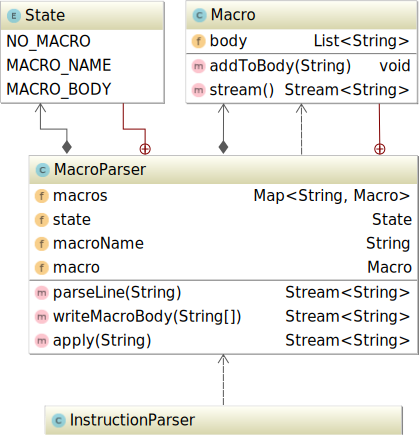
\includegraphics[scale=0.6]{svgL3/macro}
        \caption{Structure de la classe \texttt{MacroParser}}
\end{figure}

        Le traitement des macros a été ajouté avant l'analyse syntaxique des instructions, c'est à dire au début de la classe \texttt{InstructionParser}.

      En réalité, tout le traitement est dédié à la nouvelle classe \texttt{MacroParser} qui implémente l'interface fonctionnelle \texttt{Function<String, Stream<String>>}. De cette manière, l'objet \texttt{MacroParser} peut être passé directement en paramètre de la méthode \texttt{flatMap()} sur le \texttt{Stream<String>} que traite la classe \texttt{InstructionParser}. Ce \texttt{Stream}, retourné par le lecteur de fichier, contient donc les lignes du programme.


        Pour chaque ligne du fichier, si on rencontre un mot clé de définition de macro \texttt{DEFINE}, on entre dans l'état \texttt{MACRO\_NAME} qui enregistrera le nom de la macro à la ligne suivante.
        La reconnaissance du mot clé \texttt{AS} passera à l'état \texttt{MACRO\_BODY} qui déclenchera l'enregistrement du corps de la macro à partir de la ligne suivante.
        Enfin, le mot clé \texttt{END} fera revenir l'état à \texttt{NO\_MACRO}, et la macro précédemment lue sera ajoutée à une table de hachage, indéxée par son nom.
        
        La valeur dans la table de hachage correspond à un objet \texttt{Macro}, classe interne car inutile en dehors de la classe \texttt{MacroParser}.
        Cet objet comporte une liste de chaînes de caractères composant le corps de la macro, et propose une méthode \texttt{stream()} qui renvoie un \texttt{Stream<String>} construit à partir de ces lignes.

        Pendant toute la lecture de la définition d'une macro, rien n'est renvoyé.
        Dans l'état \texttt{NO\_MACRO}, la méthode \texttt{parseLine()} est appelée à chaque fois. Elle découpe la ligne au niveau de ses espaces pour récupérer le nom de la macro et son éventuel paramètre. Si une ligne est reconnue comme un nom de macro, le retour de la méthode \texttt{writeMacroBody()} est renvoyé pour dérouler la macro.
        Sinon, la ligne elle-même est renvoyée.
        
    La reconnaissance d'une macro se fait par une recherche systématique dans la table de hachage. La méthode \texttt{parseLine()} sera aussi appelée pour le corps de la macro de manière à la dérouler récursivement.

    La répétition du contenu de la macro se fait par transformation d'un \texttt{IntStream} (contenant un nombre d'entier correspondant au paramètre reçu) en \texttt{Stream<Stream<String>>}: à chaque entier correspond un \texttt{Stream<String>} qui est le corps de la macro. Le \texttt{Stream<Stream<String>>} est aplati en \texttt{Stream<String>} par un appel à \texttt{flatMap()}.

        Ce format, d'apparence verbeuse, permet d'une part une reconnaissance facile de la macro et d'autre part l'écriture du corps de la macro sur plusieurs lignes.
        À propos du paramètre de la macro, il ne permet que la répétition du contenu de la macro. Ce comportement semble suffisant puisqu'il permet de répéter autant de fois une instruction ou un bloc d'instruction que voulu. Combiné avec le déroulement récursif, cela permet d'insérer une constante dans la mémoire à l'aide l'instruction \texttt{INCR}, ou soustraire une constante avec l'instruction \texttt{DECR} par exemple.

    Comme nous utilisions déjà un traitement sur un objet \texttt{Stream<String>} auparavant, nous avons décidé de continuer dans cette voie même si ce type de traitement n'est pas des plus évident. De plus l'algorithme final ne ressemble pas tellement à du traitement fonctionnel donc l'utilisation de \texttt{Stream} n'a pas toujours de sens. En revanche des méthodes comme \texttt{flatMap()} ou \texttt{filter()} comme déjà vues simplifient certains aspects du travail. \texttt{flatMap()} permettant d'associer à un élément plusieurs éléments provenant d'un autre \texttt{Stream}, l'utiliser pour remplacer le nom d'une macro par son contenu est pertinent.


\section{Gestion du projet}


Afin de travailler sur ce niveau 3 de la manière la plus efficace possible nous avons continué d'utiliser un système de gestion de versions (\texttt{Git}) auquel nous avons ajouté l'utilisation d'un Kanban pour gérer au mieux l'avancement et la répartition des tâches. Cette répartition a été faite en début de niveau 3 afin d'attribuer chacun des points du niveau à au moins deux personnes. Cette décision a été prise dans l'optique de réduire les risques de mauvaise compréhension de l'énoncé.
De plus, nous utilisons un dépôt sur la plateforme Github pour mettre en commun nos modifications sur le code. Chacun de nous a cloné ce dépôt pour travailler dessus. Le but de cette organisation est au final de soumettre nos modifications par le biais d'une « Pull Request ». Ce principe nous permet donc de demander aux autres membres de l'équipe l'autorisation de fusionner les modifications effectuées dans le dépôt principal.

\section{Keep calm and take a step back}

La programmation orientée objet nous a beaucoup servi dans la séparation des différentes fonctionnalités de notre application. Elle nous a permis, en respectant ces principes de base (responsabilité unique des classes par exemple) de les rendre au maximum modulaire, maintenable et extensible. Toutefois, l'implémentation du comportement des instructions aurait été plus simple et plus efficace sans utiliser de classes distinctes. Un langage comme C permettant de manipuler directement des pointeurs aurait simplifié leur écriture. De la même manière, l'implémentation des métriques n'était pas intuitive en orienté objet. C'est pour cela que nous avons opté pour une énumération qui n'est pas réellement un principe conforme à la programmation orientée objet.

Lorsqu’une portion de code se répète dans le programme, les macros permettent une rédaction facilitée et améliore sa lisibilité. Le bénéfice des macros peut être mesuré empiriquement en comparant la taille du programme rédigé par le programmeur Brainfuck et la taille du programme exécuté par la machine. Supposons la macro \texttt{TO\_DIGIT} contenant 48 instructions \texttt{DECR}, 10 utilisations de la macro revient à écrire 80 caractères contre 480 caractères en syntaxe courte sans macros. La facilité d'écriture et de lecture est flagrante d'autant plus que le mot \texttt{TO\_DIGIT} a un sens sémantique contrairement aux 48 \texttt{DECR}. L'apport sémantique des macros prend tout son sens avec les macros récursives celles-ci devenant compréhensibles, de plus le rapport entre le nombre d'instructions écrites par le programmeur et le nombre réel d'instructions s'en trouve multiplié.

L'implémentation précédemment évoquée des métriques ouvre des possibilités quant à la vérification de l'exécution d'un programme Brainfuck. Elle a toutefois eu ses conséquences sur l'organisation du code lui-même : une énumération supplémentaire, ce qui nous offre de nouvelles données globales. Une modification de l'arborescence des instructions a été effectuée afin d'embarquer les fonctions liées aux métriques. Ce choix conserve l'arborescence verticale tout en regroupant les instructions aux comportements communs. 

Le coût apporté à l'interpréteur par la table de saut correspond uniquement au coût de la recherche dans cette même table. Comparé au coût de la méthode précédente, qui correspondait à un parcours inverse de toutes les instructions à chaque itération de la boucle, une recherche dans une table (et même une table de hachage dans notre cas) est bien moins coûteuse en général. Il faudrait qu'il y ait un nombre conséquent de boucles qui contiennent très peu d'instructions pour qu'on observe un désavantage côté performances.

La séparation des implémentations concernant l'analyse statique et l'analyse dynamique ne nous a pas semblé être une bonne idée d'une part car l'analyse  statique implique un programme sans condtions, ce qui rare (limitation aux programmes basiques où l'analyse ne semble pas pertinente).

Une remarque sur notre architecture à prendre en compte est le chargement total du programme en mémoire avant exécution y compris les parties exécutées une seule fois. Une amélioration de ce point nous permettrait une prise en charge de programmes bien plus long (limite de la mémoire allouée à la machine virtuelle Java).



\section{Conclusion}
En conclusion de ce niveau, notre application est fonctionnelle, livrable et implémente les nouvelles fonctionnalités qui vous ont été présentées dans ce rapport. Une majorité des apports de ce niveau concerne des améliorations pour le programmeur Brainfuck dans sa rédaction de programme et dans son travail d'analyse post-programmation (analyse de l'exécution, débogage...). 

La seule amélioration de fonctionnalités déjà présente, à savoir le support des sauts conditionnels est indirectement visible au programmeur Brainfuck (grâce aux métriques) mais se ressent surtout dans l'exécution des programmes. 

Les nouvelles fonctionnalités nous introduisent en douceur les notions et fonctionnalités qui viendront se greffer à notre projet lors de la réalisation du niveau 4. 

L'utilisation des macros est critiquable dans le sens où l'on recopie l'intégralité du contenu de la macro à chaque appel. Ce qui pourrait être intéressant serait d'accéder au contenu d'une macro directement lors de l'interprétation de la liste d'instructions. Cela éviterait de répéter le corps de la macro à chaque appel. Cette fonctionnalité sera apportée dans le niveau 4 avec les procédures.

\end{document}
